%=======================================================================
\section{Demonstration: a PCM-filled wellbore heat exchanger}
\label{sec:demo}

\subsection{Configuration}

The formulation is demonstrated on latent heat storage in the annulus of a
repurposed oil-and-gas well. A high-temperature heat pump melts the PCM during
charging and an organic Rankine cycle recovers the energy during discharging,
with pressurised water circulating through finned hairpin tubes in the borehole.
Table~\ref{tab:config} gives the configuration.

\begin{table}[htbp]
\centering
\caption{Configuration of the demonstration case.}
\label{tab:config}
\begin{tabular}{@{}l l r l@{}}
\toprule
 & quantity & value & unit \\
\midrule
\multirow{4}{*}{Borehole}
 & depth $L_{\mathrm{well}}$ & 1524 & \si{\meter} \\
 & diameter $D_{\mathrm{well}}$ & 177.8 & \si{\milli\meter} \\
 & hairpin tubes $n_{t}$ & 2 & -- \\
 & PCM volume $V_{\mathrm{well}}$ & 27.68 & \si{\meter\cubed} \\
\midrule
\multirow{4}{*}{Tube}
 & inner radius $r_{i}$ & 16.23 & \si{\milli\meter} \\
 & outer radius $r_{e}$ & 21.08 & \si{\milli\meter} \\
 & fins per leg $n_{f}$ & 24 & -- \\
 & fin $L_{f}\times t_{f}$ & $7.5\times1.5$ & \si{\milli\meter} \\
\midrule
\multirow{5}{*}{PCM}
 & melting temperature $\Tm$ & 150 & \si{\celsius} \\
 & latent heat $\hm$ & 380 & \si{\kilo\joule\per\kilogram} \\
 & $c_{p,s}$ / $c_{p,l}$ & 1280 / 1800 & \si{\joule\per\kilogram\per\kelvin} \\
 & $k_{s}$ / $k_{l}$ & 0.60 / 0.45 & \si{\watt\per\meter\per\kelvin} \\
 & $\rho_{s}$ / $\rho_{l}$ & 1550 / 1450 & \si{\kilogram\per\meter\cubed} \\
\midrule
\multirow{6}{*}{Operation}
 & fluid glide $\Delta T_{3C,2C}$ & 55 & \si{\kelvin} \\
 & charge superheat $\Delta T_{4C,M}$ & 10 & \si{\kelvin} \\
 & discharge subcooling $\Delta T_{M,1D}$ & 10 & \si{\kelvin} \\
 & charge / discharge inlet & 160.0 / 91.1 & \si{\celsius} \\
 & charge / discharge window & 10 / 10 & \si{\hour} \\
 & PCM layers $N_{\mathrm{lay}}$ & 9 & -- \\
\bottomrule
\end{tabular}
\end{table}

\noindent
The resulting capacities, Eq.~\eqref{eq:caps}, are
$\Aav=\SI{4.5411e-3}{\meter\squared}$,
$\Elat=\SI{2.675}{\mega\joule\per\meter}$,
$C_{s}=\SI{9.010e3}{\joule\per\meter\per\kelvin}$ and
$C_{l}=\SI{1.267e4}{\joule\per\meter\per\kelvin}$. The ratio
$C_{l}/\Elat=\SI{4.74e-3}{\per\kelvin}$ is the Stefan number in disguise: one
kelvin of superheat is worth \SI{0.47}{\percent} of the latent capacity, so with
the \SI{10}{\kelvin} approach nominally available the sensible branches would
appear to carry about \SI{4.7}{\percent} of the energy. A reader might
reasonably conclude that the formulation is a small correction. It is not, for
two separate reasons. The estimate itself is low --- the \SI{10}{\kelvin}
approach is the approach of the \emph{first} layer of the cascade, and a segment
that saturates goes on superheating past it, reaching \SI{18.5}{\kelvin} here,
so the measured figure is \SI{9.3}{\percent} rather than \SI{4.7}{\percent}
(Table~\ref{tab:branches}). More importantly, the energy is the wrong thing to
measure: Section~\ref{sec:levelling} shows that the sensible branches act on the
\emph{distribution} of melting, where the effect is first-order.

\subsection{The solution procedure end to end}
\label{sec:procedure}

Before the individual results, Figures~\ref{fig:proc1} and~\ref{fig:proc2}
place the formulation in the calculation that uses it. The structure is worth stating plainly because
it is unusual in one respect: \emph{nothing is solved for}. The thermodynamic
cycles, the energy budget and the exchanger size are all evaluated in sequence,
the two flow rates follow from their prescribed glides, and the only iteration
in the entire procedure is the outer loop that repeats the cycle until the store
returns to its own initial state. Section~\ref{sec:css} explains why the more
usual arrangement --- close an energy balance on the exchanger size by root
finding --- is not available once the cycle is required to repeat.

Three levels are nested. At the plant level the high-temperature heat pump and
the organic Rankine cycle are evaluated once, and their only outputs into the
rest of the calculation are two efficiencies and the secondary-fluid states that
bracket each half-cycle. They are not quite independent of the store --- the ORC
evaporating temperature follows an exchanger outlet, which is a result and not
an input (\S\ref{sec:prescribe}) --- but the dependence is weak enough to be
settled by a single correction pass rather than an outer loop. At the field
level those state points and the target duty fix how much energy must move each
cycle, and hence the number of wells. At the borehole level the segment march of
\S\ref{sec:formulation}--\S\ref{sec:integration} is executed, twice per cycle,
until the cyclic steady state is reached.

The cost is dominated by the innermost pair of loops: $n_{t}$ time levels
$\times$ $n_{s}$ segments $\times$ two half-cycles $\times$ the number of cycles
to convergence, or about $2\times10^{5}$ segment updates for the case here. Each
update is a handful of property evaluations and one closed-form advance, which
is what makes the branchwise-exact scheme worth its arithmetic: an explicit
integrator would need the time grid refined by some three orders of magnitude to
remain stable at the late steps (\S\ref{sec:integration}), and the outer loop
multiplies that cost by thirty.

\begin{figure}[tbp]
\centering
\begin{tikzpicture}[
  font=\footnotesize,
  node distance=3mm,
  blk/.style   ={draw, rounded corners=2pt, inner sep=5pt, align=left,
                 text width=0.76\linewidth},
  inp/.style   ={blk, fill=black!4},
  link/.style  ={draw, dashed, rounded corners=2pt, inner sep=4pt, align=center,
                 text width=0.60\linewidth, font=\footnotesize\itshape},
  fl/.style    ={-{Latex[length=2mm]}, thick},
  lab/.style   ={font=\scriptsize, inner sep=1.5pt}]

%------------------------------------------------------------------ inputs
\node[inp] (in) {%
  \textbf{Input specification}\\[2pt]
  \emph{duty and schedule}\ \ $\dot W_{\mathrm{el}}=\SI{1}{\mega\watt}$,
    $t_{\mathrm{ch}}=t_{\mathrm{dc}}=\SI{10}{\hour}$, two \SI{2}{\hour} rests\\
  \emph{approaches}\ \ $\Delta T_{4C,M}=\Delta T_{M,1D}=\SI{10}{\kelvin}$,
    glide $\Delta T_{3C,2C}=\SI{55}{\kelvin}$, sink/source temperatures\\
  \emph{PCM}\ \ $\Tm$, $\hm$, $c_{p,s}$, $c_{p,l}$, $k_{s}$, $k_{l}$,
    $\rho_{s}$, $\rho_{l}$, layers $N_{\mathrm{lay}}$\\
  \emph{geometry}\ \ $L_{\mathrm{well}}$, $D_{\mathrm{well}}$, $n_{t}$,
    $r_{i}$, $r_{e}$, $n_{f}$, $L_{f}$, $t_{f}$\\
  \emph{fluids}\ \ secondary water at $P$; heat-pump and ORC working fluids};

%------------------------------------------------------------------ cycles
\node[blk, below=of in] (cyc) {%
  \textbf{1.\ Thermodynamic cycles} \hfill \emph{plant level, evaluated once}\\[3pt]
  \begin{minipage}[t]{0.46\linewidth}
    \raggedright
    high-temperature heat pump\\ two stages, two regenerators\\
    $\Rightarrow\ \mathrm{COP}=2.956$
  \end{minipage}\hfill
  \begin{minipage}[t]{0.46\linewidth}
    \raggedright
    organic Rankine cycle\\ double-stage\\
    $\Rightarrow\ \eta_{\mathrm{ORC}}=0.2328$
  \end{minipage}\\[4pt]
  inlets from Eq.~\eqref{eq:inlets}: $T_{4c}=\SI{160.0}{\celsius}$,
  $T_{3d}=\SI{91.1}{\celsius}$\\
  outlets are \emph{results}; $T_{2d}$ enters here only as a provisional
  estimate, corrected once below};

%------------------------------------------------------------------ budget
\node[blk, below=of cyc] (bud) {%
  \textbf{2.\ Energy budget for one cycle} \hfill \emph{field level}\\[3pt]
  $\Delta E_{\mathrm{in,ORC}}$ from the target output and $\eta_{\mathrm{ORC}}$;
  $\Delta E_{\mathrm{out,HP}}=(1+\lambda)\,\Delta E_{\mathrm{in,ORC}}$;
  duties $\dot Q$ and the charging flow from the glide};

%------------------------------------------------------------------ hardware
\node[blk, below=of bud] (hw) {%
  \textbf{3.\ Specify the hardware} \hfill \emph{no root finding}\\[3pt]
  $\Nwells=\Delta E_{\mathrm{out,HP}}/(\rhom V_{\mathrm{well}}\hm)$
  --- latent heat alone, $\lambda=0$\\
  $\md_{\mathrm{ch}}$ and $\md_{\mathrm{dc}}$ each pinned by their own glide};

%------------------------------------------------------------------ hand-off
\node[link, below=of hw] (go) {%
  continued in Figure~\ref{fig:proc2}};

\foreach \a/\b in {in/cyc, cyc/bud, bud/hw, hw/go}
  \draw[fl] (\a) -- (\b);
\end{tikzpicture}
\caption{The solution procedure, part~1: the plant and field levels. These
blocks are evaluated once, in sequence, and nothing in them is iterated. Their
entire output into the rest of the calculation is five secondary-fluid state
points, two flow rates and a well count --- that is, a fully specified piece of
hardware. The borehole model that operates it is Figure~\ref{fig:proc2}.}
\label{fig:proc1}
\end{figure}

\begin{figure}[tbp]
\centering
\begin{tikzpicture}[
  font=\footnotesize,
  node distance=3mm,
  blk/.style   ={draw, rounded corners=2pt, inner sep=5pt, align=left,
                 text width=0.76\linewidth},
  march/.style ={blk, line width=0.9pt, fill=black!2},
  fin/.style   ={blk, fill=black!4},
  test/.style  ={draw, dashed, rounded corners=2pt, inner sep=5pt, align=center,
                 text width=0.60\linewidth},
  link/.style  ={draw, dashed, rounded corners=2pt, inner sep=4pt, align=center,
                 text width=0.60\linewidth, font=\footnotesize\itshape},
  fl/.style    ={-{Latex[length=2mm]}, thick},
  lab/.style   ={font=\scriptsize, inner sep=1.5pt}]

%------------------------------------------------------------------ hand-off
\node[link] (from) {%
  from Figure~\ref{fig:proc1}: $\Nwells$, $\md_{\mathrm{ch}}$,
  $\md_{\mathrm{dc}}$, state points};

%------------------------------------------------------------------ march
\node[march, below=of from] (mar) {%
  \textbf{4.\ Half-cycle segment march} \hfill \emph{borehole level}\\[2pt]
  charge: inlet $T_{4c}=\Tm^{\mathrm{top}}+\Delta T_{4C,M}$,
  flow $\md_{\mathrm{ch}}$\\[3pt]
  \textbf{for} each time level $t_{k}$, $k=1\ldots n_{t}$
  \ (logarithmic grid)\\
  \hspace*{3mm}\textbf{for} each segment $i=1\ldots n_{s}$, marching with the
  flow:\\
  \hspace*{7mm}(a) $\delta_{i}$ from $E'_{i}$, then the resistance network ---
  $h_{i}$ (Gnielinski),\\
  \hspace*{11mm}tube wall, fin efficiency $\etaf$, melt annulus
  $\;\Rightarrow\;\Ui$\\
  \hspace*{7mm}(b) $\mathrm{NTU}_{i}=2\pi r_{i}\Ui\Delta z/(\md c_{p})$,
  \ \ $K_{i}=\md c_{p}\bigl(1-e^{-\mathrm{NTU}_{i}}\bigr)/\Delta z$\\
  \hspace*{7mm}(c) advance $E'_{i}$ in closed form within its branch,\\
  \hspace*{11mm}splitting the step at branch crossings\\
  \hspace*{7mm}(d) fluid: $T_{i+1}=T_{i}-q'_{i}\Delta z/(\md c_{p})$};

%------------------------------------------------------------------ reversal
\node[blk, below=of mar] (rev) {%
  \textbf{5.\ Reverse the flow and discharge}\\[3pt]
  mirror the cascade \emph{and} the state, then march again with inlet
  $T_{3d}=\Tm^{\mathrm{bot}}-\Delta T_{M,1D}$ and flow $\md_{\mathrm{dc}}$.
  The two \SI{2}{\hour} rests are exact no-ops: the store is adiabatic and
  carries no axial conduction};

%------------------------------------------------------------------ test
\node[test, below=of rev] (tst) {%
  $\displaystyle\max_{i}\bigl|E'_{i}\big|_{\mathrm{end}}
   -E'_{i}\big|_{\mathrm{start}}\bigr|<\varepsilon_{\mathrm{tol}}$ ?};

%------------------------------------------------------------------ correction
\node[blk, below=6mm of tst] (corr) {%
  \textbf{6.\ Correct the ORC, once} \hfill \emph{not an outer loop}\\[3pt]
  re-evaluate $\eta_{\mathrm{ORC}}$, the budget, $\Nwells$ and both flows at the
  outlet the first pass produced, and repeat. The shift it causes is reported:
  \SI{0.002}{\kelvin} here (\S\ref{sec:prescribe})};

%------------------------------------------------------------------ outputs
\node[fin, below=of corr] (outp) {%
  \textbf{7.\ Results at cyclic steady state}\\[3pt]
  profiles of $T_{f}$, $\Tpcm$, $\varepsilon_{\mathrm{local}}$, $\Ui$ and NTU;
  melt maps over depth and time\\
  delivered $\Delta E_{\mathrm{in,ORC}}$ $\Rightarrow$ \textbf{deviation from
  the target output}\\
  round-trip and exergetic efficiencies, specific thermal and electrical
  capacity};

%------------------------------------------------------------------ arrows
\foreach \a/\b in {from/mar, mar/rev, rev/tst}
  \draw[fl] (\a) -- (\b);
\draw[fl] (tst) -- node[lab, left] {yes} (corr);
\draw[fl] (corr) -- (outp);

% CSS loop: back from the test to the march, routed clear of the blocks
\coordinate (Lx) at ($(mar.west)+(-9mm,0)$);
\draw[fl] (tst.west) -- (Lx |- tst.west)
  node[lab, midway, above] {no, \emph{next cycle}}
  -- (Lx) -- (mar.west);

\end{tikzpicture}
\caption{The solution procedure, part~2: the borehole level. Blocks~4 and~5 are
the segment march of \S\ref{sec:formulation}--\S\ref{sec:integration}, executed
twice per cycle and repeated until the store reproduces its own initial state.
That loop is the only iteration in the procedure --- block~6 runs once, and is a
second evaluation rather than a loop --- and no quantity anywhere in
Figures~\ref{fig:proc1} and~\ref{fig:proc2} is obtained by root finding, which
is a consequence of Eq.~\eqref{eq:css-unity} rather than a choice
(\S\ref{sec:css}).}
\label{fig:proc2}
\end{figure}

\subsection{Quasi-steady fluid: the cost of H7}

Table~\ref{tab:h7} collects the comparisons that justify dropping
$\partial T/\partial t$ from Eq.~\eqref{eq:fluid-pde}.

\begin{table}[htbp]
\centering
\caption{Justification and cost of the quasi-steady fluid approximation.}
\label{tab:h7}
\begin{tabular}{@{}l r l@{}}
\toprule
quantity & value & \\
\midrule
fluid transit time over $L_{\mathrm{tube}}$ & \SI{2264}{\second}
  & ($u=\SI{1.35}{\meter\per\second}$) \\
charging window $t_{\mathrm{ch}}$ & \SI{36000}{\second} & \\
ratio & \num{0.063} & \\
$\rho A_{\mathrm{flow}}c_{p}/C_{l}$ & \num{0.257}
  & fluid vs.\ PCM sensible capacity \\
$\rho A_{\mathrm{flow}}c_{p}\Delta T/\Elat$ & \num{0.0122}
  & fluid swing vs.\ latent, $\Delta T=\SI{10}{\kelvin}$ \\
\bottomrule
\end{tabular}
\end{table}

\noindent
The fluid re-establishes its profile in one transit while the PCM state evolves
over ten hours, a separation of about sixteen. The approximation is therefore
reasonable but not asymptotic: the first \SI{38}{\minute} of each half-cycle is
a startup transient the model does not resolve, some \SI{6}{\percent} of the
window. What renders this tolerable is the last row --- the energy held in the
fluid is only \SI{1.2}{\percent} of the latent inventory it is charging, so the
transient misplaces very little energy even though it occupies a noticeable
fraction of the run.

\subsection{The closure discrepancy in practice}

Over the charge, $\mathrm{NTU}$ ranges from \num{0.083} to \num{0.602}, so
Eq.~\eqref{eq:K-ratio} lies between \num{0.96} and \num{0.75}. Using
$\Ui P_{i}$ in place of Eq.~\eqref{eq:K} would therefore overstate the segment
conductance by between \SI{4}{\percent} and \SI{33}{\percent} in this case, with
the largest error at early times when the melt layer is thin and the exchanger
at its best.

\subsection{Stability of the time integration}

Table~\ref{tab:stability} gives the stability figures for the logarithmic time
grid used here.

\begin{table}[htbp]
\centering
\caption{Explicit-Euler stability limit against the time grid actually used,
for the first segment.}
\label{tab:stability}
\begin{tabular}{@{}l r r@{}}
\toprule
 & early ($t=\SI{1}{\second}$) & late ($t\to t_{\mathrm{ch}}$) \\
\midrule
$\mathrm{NTU}$ & \num{0.592} & \num{0.083} \\
$K$ [\si{\watt\per\meter\per\kelvin}] & \num{64.3} & \num{11.5} \\
$C_{l}/K$ [\si{\second}] & \num{197} & \num{1106} \\
grid step $\Delta t$ [\si{\second}] & \num{0.31} & \num{8491} \\
\midrule
$\Delta t\,K/C_{l}$ & \num{0.002} & \textbf{\num{7.7}} \\
\bottomrule
\end{tabular}
\end{table}

\noindent
The grid is comfortable at the start and violates the limit by almost an order
of magnitude at the end. An explicit implementation duly diverged, the
oscillation feeding back through the fluid temperature and driving the secondary
fluid to \SI{261}{\kelvin} --- some \SI{170}{\kelvin} below anything physical.
That failure was loud and immediately diagnosable; the dangerous case is a step
ratio nearer $1.5$, unstable in principle but slowly enough to resemble a
plausible answer.

\subsection{Sensible capacity is self-levelling}
\label{sec:levelling}

The principal physical result is not the magnitude of the sensible energy but
its effect on the \emph{distribution} of melting.

Consider the segment nearest the inlet, which sees the hottest fluid and
therefore melts first. Under an area-based formulation it finishes melting and
then continues to absorb heat at the full driving difference $T_{j}-\Tm$,
because its boundary temperature remains pinned at $\Tm$ regardless of state: it
monopolises the fluid's heat, and segments downstream receive what is left.

Under Eq.~\eqref{eq:ode} the same segment begins to superheat the instant its
solid is exhausted. $\Tpcm$ rises, the driving difference $T_{j}-\Tpcm$
collapses, its demand falls away, and the heat continues downstream to segments
that still have solid to melt. The mechanism is a negative feedback and it is
automatic --- nothing in the implementation distributes the heat, and no
parameter was tuned.

\begin{table}[htbp]
\centering
\caption{Local melted fraction at ten stations along the exchanger at end of
charge, and its spread over all \num{100} segments.}
\label{tab:levelling}
\begin{tabular}{@{}l r r r@{}}
\toprule
formulation & min & max & spread \\
\midrule
area-based (melted fraction capped) & 0.595 & 1.000 & 0.405 \\
enthalpy                            & 1.000 & 1.000 & \textbf{0.000} \\
\bottomrule
\end{tabular}
\end{table}

The comparison in Table~\ref{tab:levelling} is made at \emph{equal exchanger
size} and with the melted fraction capped in both formulations, so that only the
sensible branches differ. This matters: an unguarded area-based formulation also
produces $\varepsilon_{\mathrm{local}}$ above unity --- up to $1.78$ in this
case --- and quoting the resulting spread would conflate genuine non-uniformity
with that over-melt artefact. The figures above isolate the effect of the
sensible branches alone.

The physical reading is that PCM which never melts is dead volume, occupying the
store and carrying no energy through the round trip. The enthalpy formulation
finds substantially less of it.

Figure~\ref{fig:levelling} shows why the summary statistics understate the
effect. The area-based curve is not uniformly depressed; it is a \emph{sawtooth}
locked to the cascade. Each layer melts completely at its inlet end, where the
fluid is \SI{10}{\kelvin} above that layer's $\Tm$, and incompletely at its
outlet end, because segments upstream that have already finished continue to
draw heat at the full driving difference and leave less for those behind. The
enthalpy formulation removes the sawtooth rather than merely shifting its mean:
a segment that finishes melting superheats, its own driving difference
collapses, and the heat is passed along.
%---------------------------------------------------------------------
\begin{figure}[htbp]
\centering
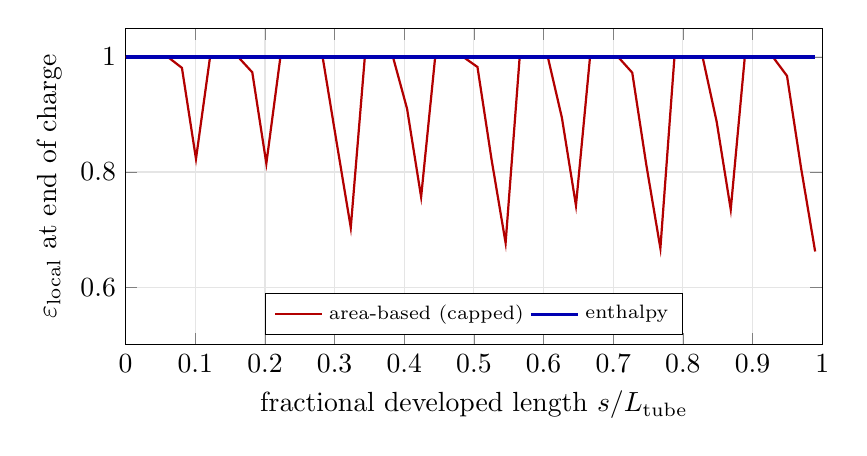
\begin{tikzpicture}
\begin{axis}[width=0.86\linewidth,height=5.6cm,
  xlabel={fractional developed length $s/L_{\mathrm{tube}}$},
  ylabel={$\varepsilon_{\mathrm{local}}$ at end of charge},
  ymin=0.5, ymax=1.05, xmin=0, xmax=1,
  legend style={font=\scriptsize,at={(0.5,0.03)},anchor=south},
  legend columns=2, grid=both, grid style={gray!20}]
\addplot[thick,red!70!black] coordinates {(0,1.0000) (0.0202,1.0000) (0.0404,1.0000) (0.06061,1.0000) (0.08081,0.9811) (0.101,0.8229) (0.1212,1.0000) (0.1414,1.0000) (0.1616,1.0000) (0.1818,0.9734) (0.202,0.8149) (0.2222,1.0000) (0.2424,1.0000) (0.2626,1.0000) (0.2828,1.0000) (0.303,0.8509) (0.3232,0.7034) (0.3434,1.0000) (0.3636,1.0000) (0.3838,1.0000) (0.404,0.9102) (0.4242,0.7567) (0.4444,1.0000) (0.4646,1.0000) (0.4848,1.0000) (0.5051,0.9826) (0.5253,0.8220) (0.5455,0.6768) (0.5657,1.0000) (0.5859,1.0000) (0.6061,1.0000) (0.6263,0.8945) (0.6465,0.7419) (0.6667,1.0000) (0.6869,1.0000) (0.7071,1.0000) (0.7273,0.9728) (0.7475,0.8124) (0.7677,0.6675) (0.7879,1.0000) (0.8081,1.0000) (0.8283,1.0000) (0.8485,0.8875) (0.8687,0.7349) (0.8889,1.0000) (0.9091,1.0000) (0.9293,1.0000) (0.9495,0.9671) (0.9697,0.8068) (0.9899,0.6619)};
\addlegendentry{area-based (capped)}
\addplot[very thick,blue!70!black] coordinates {(0,1.0000) (0.0202,1.0000) (0.0404,1.0000) (0.06061,1.0000) (0.08081,1.0000) (0.101,1.0000) (0.1212,1.0000) (0.1414,1.0000) (0.1616,1.0000) (0.1818,1.0000) (0.202,1.0000) (0.2222,1.0000) (0.2424,1.0000) (0.2626,1.0000) (0.2828,1.0000) (0.303,1.0000) (0.3232,1.0000) (0.3434,1.0000) (0.3636,1.0000) (0.3838,1.0000) (0.404,1.0000) (0.4242,1.0000) (0.4444,1.0000) (0.4646,1.0000) (0.4848,1.0000) (0.5051,1.0000) (0.5253,1.0000) (0.5455,1.0000) (0.5657,1.0000) (0.5859,1.0000) (0.6061,1.0000) (0.6263,1.0000) (0.6465,1.0000) (0.6667,1.0000) (0.6869,1.0000) (0.7071,1.0000) (0.7273,1.0000) (0.7475,1.0000) (0.7677,1.0000) (0.7879,1.0000) (0.8081,1.0000) (0.8283,1.0000) (0.8485,1.0000) (0.8687,1.0000) (0.8889,1.0000) (0.9091,1.0000) (0.9293,1.0000) (0.9495,1.0000) (0.9697,1.0000) (0.9899,1.0000)};
\addlegendentry{enthalpy}
\end{axis}
\end{tikzpicture}
\caption{Local melted fraction along the exchanger at end of charge, compared
at \emph{equal} exchanger size with the melted fraction capped in both
formulations. The sawtooth in the area-based curve is the cascade: each layer
melts fully at its inlet end and incompletely at its outlet end, because a
segment that has finished melting continues to draw heat at the full driving
difference. Under the enthalpy formulation that segment superheats instead, its
demand collapses, and the heat passes downstream --- the curve is flat at
unity. Spread falls from $0.405$ to $0.000$ (Table~\ref{tab:levelling}).}
\label{fig:levelling}
\end{figure}



\subsection{Cyclic steady state}
\label{sec:css}

The results above are \emph{first-cycle} results: the store begins fully solid
at $\Tm$ and the cycle does not return to that state. Repeating the
charge--discharge schedule drives the store to a cyclic steady state (CSS) in
which the end-of-cycle state reproduces the start-of-cycle state. Convergence
takes of order thirty cycles here.

At CSS the enthalpy change over a complete cycle is zero by definition, and the
store is adiabatic, so
\begin{equation}
  \eta_{\mathrm{storage}}(\mathrm{CSS}) \;\equiv\; 1
  \label{eq:css-unity}
\end{equation}
identically --- for every exchanger size and every flow rate; computed values
agree to eight decimal places. Equation~\eqref{eq:css-unity} is energy
conservation applied to a closed cycle rather than a result about the store, but
it has a consequence for how such a model may be posed.

\paragraph{How much of the throughput the plateau cannot carry.}
A repeating cycle is also the cleanest setting in which to measure what
\S\ref{sec:intro} argued structurally, because the state returns to itself and
the charge and discharge must therefore give the same answer. Decomposing the
enthalpy change of every segment over a half-cycle into the part traversed
within the two-phase plateau, $0\le E'\le\Elat$, and the parts traversed outside
it gives Table~\ref{tab:branches}. Just over a tenth of the energy passing
through the store is carried by the sensible branches, and it is not optional:
at the end of the charge \emph{all} \num{100} segments stand at
$\varepsilon_{\mathrm{local}}=1$, with a peak superheat of \SI{18.5}{\kelvin},
so a formulation whose state stops at $\Tm$ has nowhere to put the last
\SI{7.1}{\percent} of the charge and nothing to draw the corresponding part of
the discharge from.

\begin{table}[htbp]
\centering
\caption{Decomposition of the enthalpy change of the store over a half-cycle at
cyclic steady state, by the branch of Eq.~\eqref{eq:enth-curve} traversed.
Charge and discharge agree exactly, as Eq.~\eqref{eq:css-unity} requires.}
\label{tab:branches}
\begin{tabular}{@{}l r r@{}}
\toprule
branch & \% of half-cycle energy & peak departure from $\Tm$ \\
\midrule
two-phase plateau, $0\le E'\le\Elat$ & 90.66 & --- \\
superheated liquid, $E'>\Elat$       &  7.09 & \SI{18.5}{\kelvin} \\
subcooled solid, $E'<0$              &  2.25 & \SI{11.5}{\kelvin} \\
\midrule
outside the plateau                  & \textbf{9.34} & \\
\bottomrule
\end{tabular}
\end{table}

\paragraph{Sizing cannot be closed on the energy balance at CSS.}
A single-cycle model sizes the exchanger by requiring that it absorb a specified
energy within the charging window. At CSS the absorbed and recovered energies
are the \emph{same number}, so that requirement and the corresponding discharge
requirement collapse into one equation. It fixes the ratio of the two flow rates
and says nothing about the exchanger size:

\begin{center}
\begin{tabular}{@{}r r r r@{}}
\toprule
$\Nwells$ & flow ratio & charge/target & discharge/target \\
\midrule
11.0 & 1.0740 & 1.00000 & 1.00000 \\
14.0 & 1.0280 & 0.99994 & 0.99994 \\
20.0 & 0.9965 & 0.99994 & 0.99994 \\
\bottomrule
\end{tabular}
\end{center}

\noindent
Adding a loss mechanism would not remove this degeneracy: at CSS the charge
would then exceed the discharge by exactly the loss, and the one remaining
equation would still pin the flow ratio.

\paragraph{Reformulation.}
The resolution is to specify the hardware and \emph{simulate} rather than solve.
The exchanger count is taken from the latent inventory alone,
$\Delta E/(\rhom V_{\mathrm{well}}\hm)$ --- a deliberate overestimate, since it
ignores the sensible capacity the store also has --- and both flows are pinned
by their specified glides. No quantity is solved for, so no convergence question
arises, and the deviation of delivered energy from target becomes a reported
result.

\begin{table}[htbp]
\centering
\caption{Cyclic steady state: deviation from target against exchanger count.
Each row is an independent march to CSS.}
\label{tab:css}
\begin{tabular}{@{}r r r r@{}}
\toprule
$\Nwells$ & delivered/target & $\varepsilon$ end charge & $\varepsilon$ end discharge \\
\midrule
11.544 & 0.9426 & 1.000 & 0.154 \\
14.000 & 0.9662 & 1.000 & 0.288 \\
16.000 & 0.9777 & 1.000 & 0.376 \\
20.000 & 0.9931 & 1.000 & 0.505 \\
26.000 & 1.0082 & 1.000 & 0.629 \\
\bottomrule
\end{tabular}
\end{table}

%---------------------------------------------------------------------
\begin{figure}[htbp]
\centering
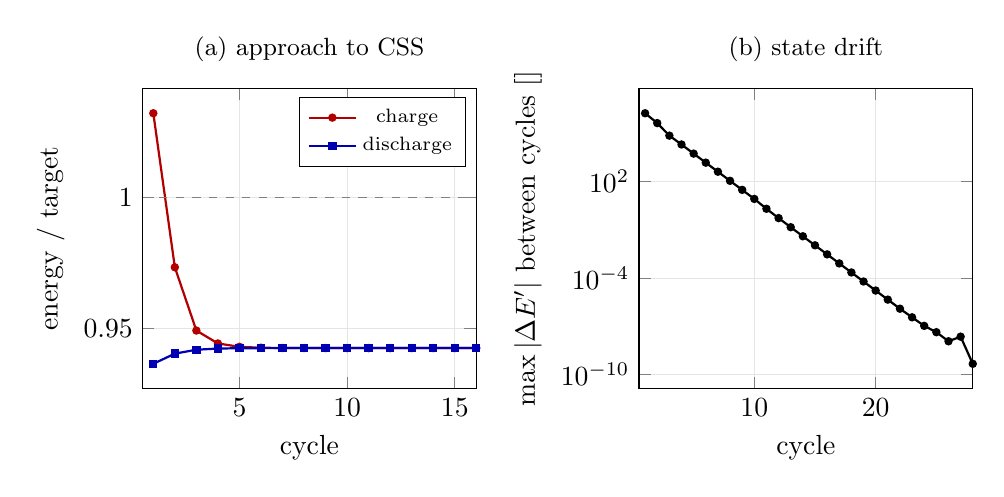
\begin{tikzpicture}
\begin{axis}[width=0.48\linewidth,height=5.4cm,
  xlabel={cycle}, ylabel={energy / target}, xmin=0.5, xmax=16,
  title={\small (a) approach to CSS},
  legend style={font=\scriptsize,at={(0.97,0.97)},anchor=north east},
  grid=both, grid style={gray!20}]
\addplot[thick,mark=*,mark size=1.1pt,red!70!black] coordinates {(1,1.03215) (2,0.97343) (3,0.94932) (4,0.94440) (5,0.94312) (6,0.94277) (7,0.94267) (8,0.94265) (9,0.94264) (10,0.94264) (11,0.94264) (12,0.94264) (13,0.94264) (14,0.94264) (15,0.94264) (16,0.94264) (17,0.94264) (18,0.94264) (19,0.94264) (20,0.94264) (21,0.94264) (22,0.94264) (23,0.94264) (24,0.94264) (25,0.94264) (26,0.94264) (27,0.94264) (28,0.94264)};
\addlegendentry{charge}
\addplot[thick,mark=square*,mark size=1.1pt,blue!70!black] coordinates {(1,0.93665) (2,0.94052) (3,0.94201) (4,0.94246) (5,0.94259) (6,0.94262) (7,0.94263) (8,0.94264) (9,0.94264) (10,0.94264) (11,0.94264) (12,0.94264) (13,0.94264) (14,0.94264) (15,0.94264) (16,0.94264) (17,0.94264) (18,0.94264) (19,0.94264) (20,0.94264) (21,0.94264) (22,0.94264) (23,0.94264) (24,0.94264) (25,0.94264) (26,0.94264) (27,0.94264) (28,0.94264)};
\addlegendentry{discharge}
\addplot[dashed,gray,domain=0.5:16,samples=2,forget plot] {1};
\end{axis}
\begin{axis}[width=0.48\linewidth,height=5.4cm,at={(0.52\linewidth,0)},
  xlabel={cycle}, ylabel={$\max|\Delta E'|$ between cycles [\si{\joule\per\meter}]},
  ymode=log, title={\small (b) state drift}, xmin=0.5, xmax=28,
  grid=both, grid style={gray!20}]
\addplot[thick,mark=*,mark size=1.1pt,black] coordinates {(1,1.8176e+06) (2,4.4441e+05) (3,7.3527e+04) (4,2.0698e+04) (5,5.5899e+03) (6,1.5284e+03) (7,4.1826e+02) (8,1.1346e+02) (9,3.1015e+01) (10,8.4881e+00) (11,2.0663e+00) (12,5.4292e-01) (13,1.4715e-01) (14,4.0183e-02) (15,1.0989e-02) (16,3.0059e-03) (17,8.2231e-04) (18,2.2496e-04) (19,6.1545e-05) (20,1.6842e-05) (21,4.5870e-06) (22,1.2470e-06) (23,3.6345e-07) (24,1.0675e-07) (25,4.3190e-08) (26,1.1758e-08) (27,2.2817e-08) (28,4.6566e-10)};
\end{axis}
\end{tikzpicture}
\caption{Convergence to cyclic steady state at the latent-only exchanger count.
(a) The first cycle is the outlier: it starts from a cold, fully solid store and
absorbs more than any later cycle. Charge and discharge converge to the
\emph{same} value, which is Eq.~\eqref{eq:css-unity} in practice --- the two
curves become indistinguishable, not merely close. (b) The state drift falls
geometrically; the run is stopped at $10^{-9}$.}
\label{fig:cssconv}
\end{figure}


Figure~\ref{fig:cssconv}(a) is worth dwelling on. The charge curve starts
\emph{above} target and falls; the discharge curve starts below and rises; they
meet. That meeting is not a numerical coincidence but
Eq.~\eqref{eq:css-unity} asserting itself: once the state repeats, the two
energies are the same number. The first cycle absorbs more than any later one
because it alone begins from a cold, fully solid store --- which is precisely
why a first-cycle result cannot be quoted for a repeating duty.

At the latent-only size the field delivers \SI{101.23}{\percent} of target. The
store melts \emph{completely} at end of charge --- $\varepsilon_{\mathrm{local}}
= 1.000$ at every station --- but returns only to a mean of $0.082$, so what
limits it is the \textbf{discharge rate} rather than the inventory. The
signature is in the last column, drawn in Fig.~\ref{fig:cssdesign}: the residual
melt fraction \emph{rises} with exchanger count, because each unit is then
worked less hard and proportionally less of it refreezes. Were the limit an
inventory limit it would fall, since a larger store would be proportionally
emptier at the end of a fixed discharge. The two curves therefore separate the
two failure modes without any additional calculation, and they place the lever
on the discharge side --- flow rate, window length, or conductance --- rather
than on more phase-change material.
%---------------------------------------------------------------------
\begin{figure}[htbp]
\centering
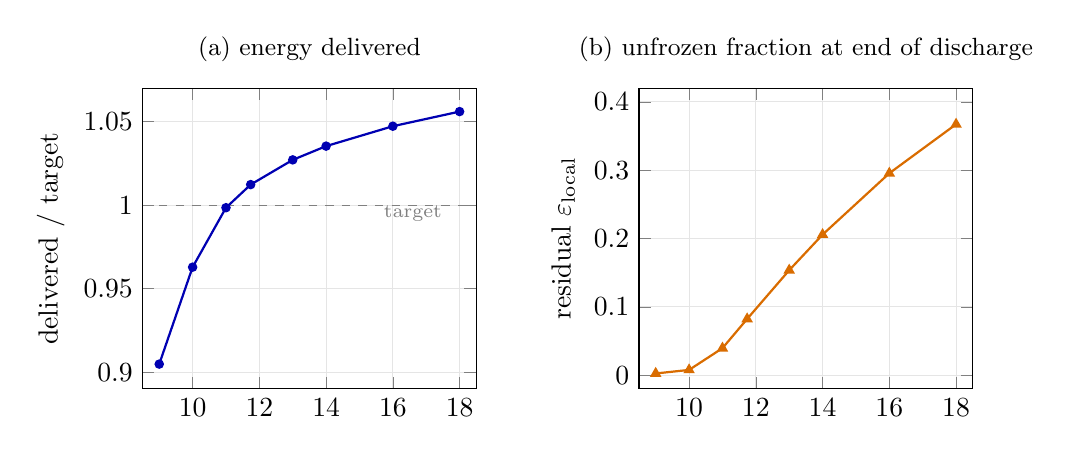
\begin{tikzpicture}
\begin{axis}[width=0.48\linewidth,height=5.4cm,
  xlabel={$\Nwells$}, ylabel={delivered / target},
  title={\small (a) energy delivered}, ymin=0.89, ymax=1.07, xmin=8.5, xmax=18.5,
  grid=both, grid style={gray!20}]
\addplot[thick,mark=*,mark size=1.3pt,blue!70!black] coordinates {(9.00,0.90481) (10.00,0.96284) (11.00,0.99845) (11.74,1.01228) (13.00,1.02708) (14.00,1.03531) (16.00,1.04723) (18.00,1.05599)};
\addplot[dashed,gray,domain=8.5:18.5,samples=2,forget plot] {1};
\node[font=\scriptsize,gray] at (axis cs:16.6,0.995) {target};
\end{axis}
\begin{axis}[width=0.48\linewidth,height=5.4cm,at={(0.52\linewidth,0)},
  xlabel={$\Nwells$},
  ylabel={residual $\varepsilon_{\mathrm{local}}$},
  title={\small (b) unfrozen fraction at end of discharge},
  ymin=-0.02, ymax=0.42, xmin=8.5, xmax=18.5,
  grid=both, grid style={gray!20}]
\addplot[thick,mark=triangle*,mark size=1.6pt,orange!85!black] coordinates {(9.00,0.0025) (10.00,0.0077) (11.00,0.0395) (11.74,0.0823) (13.00,0.1536) (14.00,0.2057) (16.00,0.2955) (18.00,0.3672)};
\end{axis}
\end{tikzpicture}
\caption{Cyclic steady state against exchanger count; each point is an
independent march to convergence. (a) Delivered energy crosses target near
$\Nwells\approx11.0$, slightly \emph{below} the latent-only count of $11.74$.
(b) The diagnostic: the
residual melted fraction at end of discharge \emph{rises} with exchanger count,
because each unit is then worked less hard and proportionally less of it
refreezes. An inventory-limited store would show the opposite, since a larger
store would be proportionally emptier after a fixed discharge. Note that the two
panels carry different quantities on similar-looking curves; they are plotted
separately for that reason.}
\label{fig:cssdesign}
\end{figure}


\subsection{What the formulation forbids you to prescribe}
\label{sec:prescribe}

A formulation that lets the phase-change material leave $\Tm$ also takes away a
boundary condition that area-based models could get away with, and the point
generalises beyond this case.

Only the two exchanger \emph{inlets} are boundary conditions on the march. Both
outlets are results of the heat transfer. An area-based model can blur this,
because a saturated control volume holds its surface at $\Tm$ and the outlet
temperature is then bounded by the cascade whatever happens. Under
Eq.~\eqref{eq:enth-curve} it is not: the store finishes each charge superheated,
so at the start of the following discharge the water leaves the exchanger at
\SI{157.93}{\celsius}, nearly \SI{8}{\kelvin} \emph{above} the melting
temperature of the hottest layer. Any prescribed value for that outlet is
contradicted by the solution.

The demonstration case originally carried exactly this defect. The discharge was
closed by pinning the outlet at the top layer's melting temperature and deriving
the inlet from it by subtracting the glide, which made the inlet approach
\begin{equation}
  \Delta T_{\mathrm{implied}}
  =\frac{\Delta T_{3C,2C}}{N_{\mathrm{lay}}}=\SI{6.111}{\kelvin},
  \label{eq:implied}
\end{equation}
one layer width --- a number nobody chose, and one that moves silently with the
number of layers. The repair is to prescribe the two inlets symmetrically, as
the approaches they are:
\begin{equation}
  T_{\mathrm{in}}^{\mathrm{ch}}=\Tm^{\mathrm{top}}+\Delta T_{4C,M},
  \qquad
  T_{\mathrm{in}}^{\mathrm{dc}}=\Tm^{\mathrm{bot}}-\Delta T_{M,1D},
  \label{eq:inlets}
\end{equation}
with $\Tm^{\mathrm{bot}}=\Tm^{\mathrm{top}}
-\Delta T_{3C,2C}(N_{\mathrm{lay}}-1)/N_{\mathrm{lay}}$ the coldest layer, which
is the end the discharge enters. The outlet becomes a reported result.

This matters quantitatively. Taking $\Delta T_{M,1D}=\SI{10}{\kelvin}$, the
symmetric partner of the charging superheat rather than an accident of
Eq.~\eqref{eq:implied}, moves the deviation of delivered energy from
\SI{-5.69}{\percent} to \SI{+1.23}{\percent}: most of what looked like a
shortfall of the store was a property of the closure. Setting
$\Delta T_{M,1D}=\Delta T_{3C,2C}/N_{\mathrm{lay}}$ reproduces the earlier
results to the last bit, so the change is a reparameterisation and the
difference above is entirely the choice of approach.

\paragraph{The cost, and why it is small.}
The ORC evaporating temperature is tied to the exchanger outlet, so demoting
that outlet to a result couples the plant to the store --- the decoupling that
Figure~\ref{fig:proc1} relies on. The coupling is weak in a specific and
checkable sense: the outlet is set by the store, not by the plant. Over a sweep
of $\Delta T_{M,1D}$ from \SI{6}{\kelvin} to \SI{15}{\kelvin}, which moves the
inlet by \SI{9}{\kelvin} and the deviation by twelve percentage points, the
realised outlet moves by less than \SI{0.3}{\kelvin}. One correction pass ---
evaluate the ORC at the outlet the first pass produced, then repeat --- shifts
it by at most \SI{0.03}{\kelvin}, so no outer iteration is needed and the
procedure of Figures~\ref{fig:proc1} and~\ref{fig:proc2} keeps its single loop.
The shift is reported rather than assumed; if it were ever large, the remedy
would be to iterate.

\paragraph{A caution on what to do with the freedom.}
The deviation crosses zero at $\Delta T_{M,1D}\approx\SI{9.30}{\kelvin}$. That
value is deliberately \emph{not} adopted. Choosing an approach because it zeroes
the deviation converts the one honestly reported output of the procedure back
into a satisfied constraint, which is precisely the move \S\ref{sec:css} argues
against. \SI{10}{\kelvin} is adopted because it is symmetric with the charge.

\subsection{Consequence for sizing}

Because the formulation conserves energy and bounds the melted fraction, the
store may be sized against two independent requirements rather than one. Writing
$\Delta E$ for the energy to be stored, the field must both \emph{absorb} it
within the charging window and \emph{contain} it at all:
\begin{equation}
  \Nwells = \max\bigl(N_{\mathrm{rate}},\,N_{\mathrm{capacity}}\bigr),
  \qquad
  N_{\mathrm{capacity}} = \frac{\Delta E}
  {\rhom V_{\mathrm{well}}\left[\hm+c_{p,l}\Delta T\right]}.
  \label{eq:sizing}
\end{equation}
$N_{\mathrm{rate}}$ follows from a root solve on the march and carries every
thermal parameter; $N_{\mathrm{capacity}}$ is closed form and carries none, which
makes it a hard lower bound no design can better. This applies to the
\emph{first} cycle; \S\ref{sec:css} shows that the rate criterion does not
survive the passage to cyclic steady state.

%=======================================================================
\section{Conclusions}
\label{sec:conclusions}

A lumped enthalpy state has been formulated for phase-change material in the
segments of a one-dimensional heat exchanger model, together with the closure
that couples it to an effectiveness--NTU march and an exact time integrator for
the resulting equation.

\begin{enumerate}[leftmargin=1.8em,itemsep=3pt]
\item Carrying enthalpy rather than melted area removes a structural defect in
  reduced-order latent storage models. A segment whose phase change is complete
  has somewhere to put further heat, so none is discarded and the melted
  fraction is confined to $[0,1]$ by the constitutive relation rather than by a
  guard. The amount at stake is not small: at cyclic steady state the store
  finishes each charge fully molten in all \num{100} segments, with a peak
  superheat of \SI{18.5}{\kelvin}, and \SI{9.3}{\percent} of the energy
  passing through the store each cycle traverses the sensible branches ---
  \SI{7.1}{\percent} as superheat and \SI{2.3}{\percent} as subcooling. That is
  the energy an area-based state must either discard or fabricate.
\item The conductance closing the segment equation is
  $K=\md c_{p}(1-e^{-\mathrm{NTU}})/\Delta z$ and not $\Ui P_{i}$. The two agree
  only as $\mathrm{NTU}\to0$, differ by \SI{4}{\percent} to \SI{33}{\percent}
  over the case studied, and only the former carries the capacity-rate limit
  that prevents heat flowing from cold to hot as the wall conductance improves.
\item Explicit time stepping is exact on the latent plateau and inadmissible off
  it, which is why area-based formulations never encountered the constraint. The
  branchwise-exact scheme of \S\ref{sec:integration} is unconditionally stable,
  makes energy closure structural, and agrees with a \num{200000}-substep
  reference to $3\times10^{-13}$.
\item Sensible capacity is self-levelling. Although it carries only about
  \SI{4.7}{\percent} of the energy in the case studied, it redistributes the
  melting: compared at equal exchanger size, the spread in local melted fraction
  falls from $0.405$ to $0.000$ and dead volume falls correspondingly. The
  effect is first-order in the distribution while being small in the energy,
  because it acts through the driving temperature difference rather than through
  the energy stored.
\item At cyclic steady state the recovered-to-stored energy ratio is identically
  unity in an adiabatic store (\S\ref{sec:css}), which collapses the charge and
  discharge energy requirements into a single equation. That equation fixes the
  ratio of the two flow rates and leaves the exchanger size undetermined, so a
  single-cycle sizing procedure does not carry over. Posing the problem as a
  simulation --- specify the hardware, march to CSS, report the deviation from
  target --- removes the difficulty rather than working around it, and turns the
  residual melt fraction into a diagnostic that distinguishes a rate limit from
  an inventory limit.
\end{enumerate}

\paragraph{Limitations.}
Three assumptions bound the results above and are stated here rather than left
implicit. Hypothesis H3 is \emph{saturated} at the design point: the melt fronts
of neighbouring tubes are in contact over \SI{99}{\percent} of the exchanger, so
the annular conduction resistance is evaluated at the limit of its validity and
the residual solid --- which occupies the corners between tubes, on a longer and
narrower conduction path than an annulus represents --- has its resistance
understated. Hypothesis H6 assumes the cell boundary adiabatic, which for an
axially graded store requires a physical partition between layers that are, at
the inlet end of the case studied, \SI{48.9}{\kelvin} apart; a slab estimate
places the neglected cross-boundary leak at some \SI{25}{\percent} of the useful
duty, and it flows in the direction that erodes the grading. Finally, the time
grid is not converged: $\varepsilon_{\mathrm{PCM}}$ moves $-0.3\,\%$ between
\num{40} and \num{320} time levels, one-sided. The first two are geometric
questions about a cell's outer boundary and would be settled together by a
two-dimensional conduction calculation on the real cross-section, which is the
natural next step. None of the three affects the formulation or the integrator,
which are the subject of this paper; all three affect the quantitative results
of \S\ref{sec:demo}, which should accordingly be read as optimistic. In
particular the \SI{-5.7}{\percent} cyclic-steady-state deviation of
\S\ref{sec:css} sits inside the band those three assumptions span, and is
better read as evidence that the store is discharge-rate limited than as a
calibrated shortfall.

%=======================================================================
\section*{Nomenclature}

\noindent
\begin{tabular}{@{}l l l@{}}
$\Amelt$ & melted cross-section per unit tube length & \si{\meter\squared} \\
$\Aav$ & PCM cross-section owned by one segment & \si{\meter\squared} \\
$A_{\mathrm{flow}}$ & tube flow area & \si{\meter\squared} \\
$c_{p}$ & specific heat capacity & \si{\joule\per\kilogram\per\kelvin} \\
$C_{s},C_{l}$ & sensible capacity per unit tube length & \si{\joule\per\meter\per\kelvin} \\
$E'$ & PCM enthalpy per unit tube length & \si{\joule\per\meter} \\
$\Elat$ & latent capacity per unit tube length & \si{\joule\per\meter} \\
$\Eeq$ & equilibrium enthalpy & \si{\joule\per\meter} \\
$\hm$ & latent heat of fusion & \si{\joule\per\kilogram} \\
$h_{e},h_{i}$ & outer, inner heat transfer coefficient & \si{\watt\per\meter\squared\per\kelvin} \\
$K$ & segment conductance per unit tube length & \si{\watt\per\meter\per\kelvin} \\
$\km,k_{w}$ & PCM, wall thermal conductivity & \si{\watt\per\meter\per\kelvin} \\
$L_{f},t_{f},n_{f}$ & fin length, thickness, count & \si{\meter},\si{\meter},-- \\
$\md$ & mass flow rate & \si{\kilogram\per\second} \\
$\mathrm{NTU}$ & number of transfer units per segment & -- \\
$P_{T}$ & finned outer perimeter & \si{\meter} \\
$q'$ & heat rate per unit tube length & \si{\watt\per\meter} \\
$r_{i},r_{e}$ & tube inner, outer radius & \si{\meter} \\
$s$ & developed tube coordinate & \si{\meter} \\
$\mathrm{Ste}$ & Stefan number, $c_{p}\Delta T/\hm$ & -- \\
$T$ & fluid temperature & \si{\kelvin} \\
$\Tm,\Tpcm$ & melting, PCM temperature & \si{\kelvin} \\
$\Ui$ & overall coefficient on inner area & \si{\watt\per\meter\squared\per\kelvin} \\
$\Delta z$ & segment length & \si{\meter} \\
$\delta$ & melt-layer thickness & \si{\meter} \\
$\varepsilon_{\mathrm{local}}$ & melted fraction of one segment & -- \\
$\etaf,\etao$ & fin, overall surface efficiency & -- \\
$\rhom$ & PCM density & \si{\kilogram\per\meter\cubed} \\
\end{tabular}

